\documentclass[10pt,a4paper]{labreport}
\usepackage{csquotes}
\usepackage{titlesec}
\usepackage{ragged2e}
\usepackage{siunitx}
\usepackage{setspace}
\usepackage{longtable}
\usepackage{rotating}
\usepackage{xurl}
\usepackage{physics}
\usepackage{caption}
\usepackage{wrapfig}
\usepackage{tabularray}
\usepackage{fancyhdr}
\usepackage{subcaption}
\usepackage{lscape}
\usepackage{tensor}
\usepackage{multirow}
\usepackage{chemformula}
\usepackage[gen]{eurosym}
\usepackage{float}
\usepackage{bm}
\usepackage{lipsum}
\usepackage{parskip}
\usepackage{booktabs}
\usepackage{enumerate}
\usepackage[justification=justified]{caption}
\usepackage[nottoc]{tocbibind}
\usepackage{color}

\usepackage{listings}
\definecolor{codegreen}{rgb}{0,0.6,0}
\definecolor{codegray}{rgb}{0.5,0.5,0.5}
\definecolor{codepurple}{rgb}{0.58,0,0.82}
\definecolor{backcolour}{rgb}{0.95,0.95,0.92}
\lstdefinestyle{mystyle}{
    backgroundcolor=\color{backcolour},   
    commentstyle=\color{codegreen},
    keywordstyle=\color{codepurple},
    numberstyle=\tiny\color{codegray},
   % stringstyle=\color{grey},
    basicstyle=\ttfamily\footnotesize,
    breakatwhitespace=false,         
    breaklines=true,                 
    captionpos=b,                    
    keepspaces=true,                 
    numbers=left,                    
    numbersep=5pt,                  
    showspaces=false,                
    showstringspaces=false,
    showtabs=false,                  
    tabsize=5
}
\lstset{style=mystyle}
\usepackage{hyperref}
 \usepackage[
backend=biber,
style=chem-acs,articletitle=true,doi=true]{biblatex}
\addbibresource{references.bib}





\title{Nanoscale Material Modeling
\\
\normalsize{Week 3}} % Main title and sub title. 

\author{Ilija A. Gjerapić, S4437586; \href{mailto:i.a.gjerapic@student.rug.nl}{i.a.gjerapic@student.rug.nl}; \href{https://github.com/igjerapic/nmm-week3/}{@github} } % Name, student number, email

\supervisors{prof. dr. A. Giuntoli, prof. dr. J. Slawinska}

\begin{document}


\maketitle

\tableofcontents

  

\thispagestyle{firststyle}
\newpage
\section{Assignment 1: DFT calculation of WTe2 monolayer}
\subsection{Structure visualization}

Figure \ref{fig:ass1_cryst} shows the \texttt{xcrysden} visulation of the \texttt{wte2.scf.in} input file. It is clear that the structure has a rectangular Bravais lattice. 

The structure is constructed by first generating a orthorhombic supercell using the \texttt{ibrav=0} command and specifying the cell size later under the \texttt{CELL\_PARAMETERS} section. The final cell has dimensions of 3.5, 6.25, and 30 {\AA} in the  $x$-, $y$- and $z$- directions, respectively.

The atom positions are then provided with respect to the Cartesian coordinate system.

  \begin{figure}[h]
    \centering 
    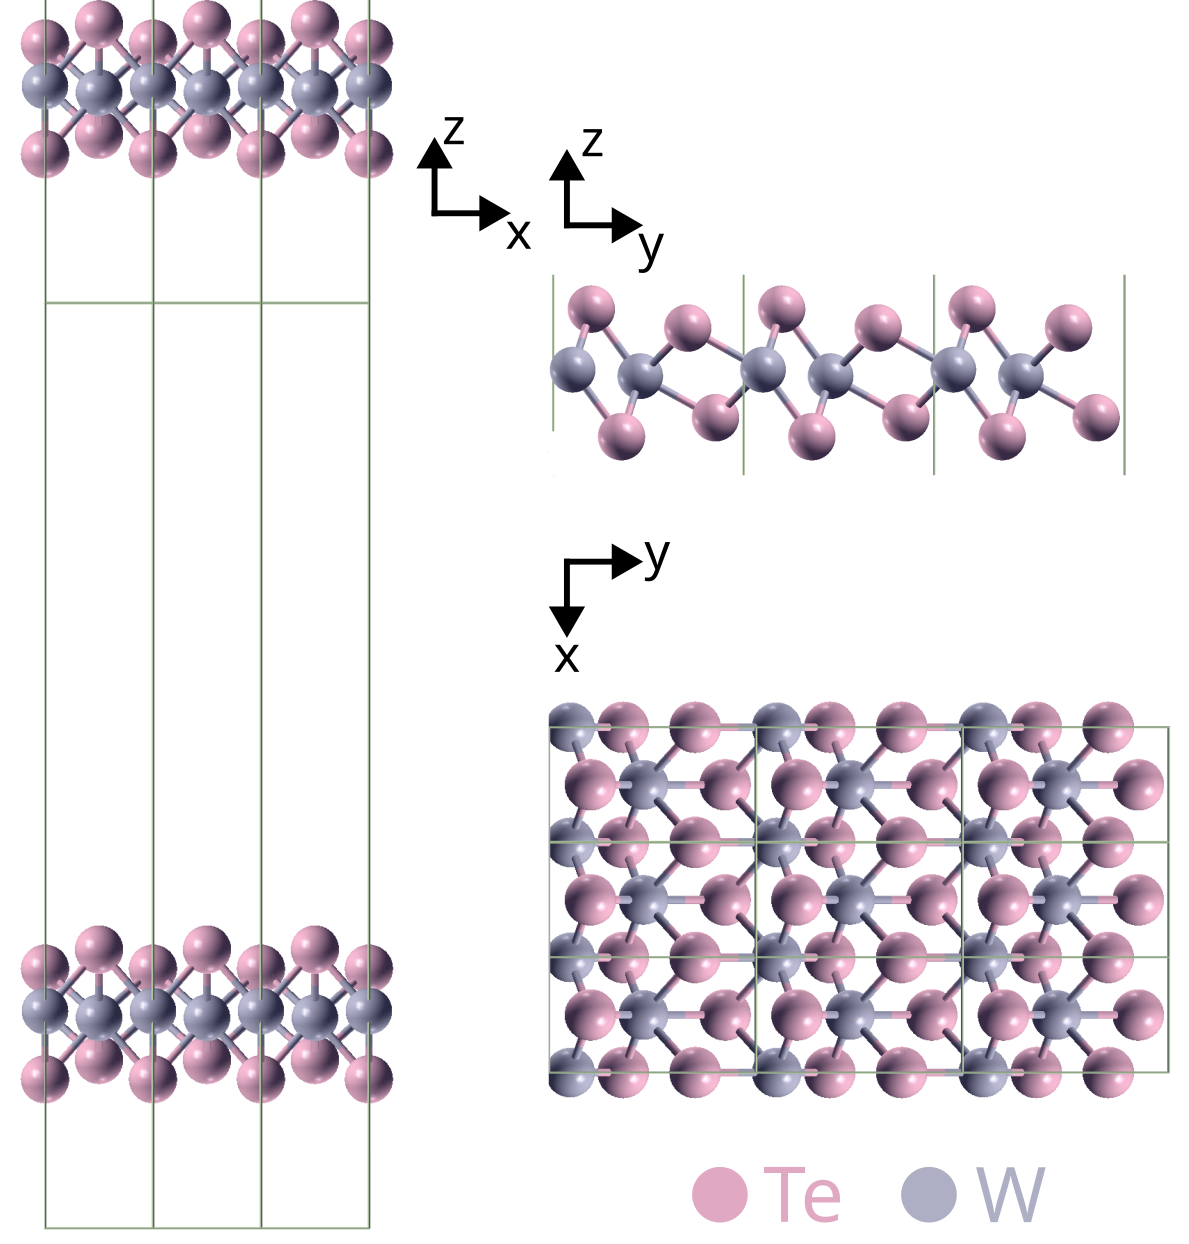
\includegraphics[width = 0.7\textwidth]{figs/ass1_WTe2_struct.png}
    \caption{The \texttt{xcrysden} visualization of the WTe2 monolayer. The distance between two monolayers is 30 \AA. as provided in the input file. }
    \label{fig:ass1_cryst}
  \end{figure}

\newpage
\subsection{Band Structure}
The high-symmetry point path chosen to outline the electronic structure of WTe2 monolayer is shown in Figure \ref{fig:ass1_kpoints}
\begin{figure}[h]
    \centering 
    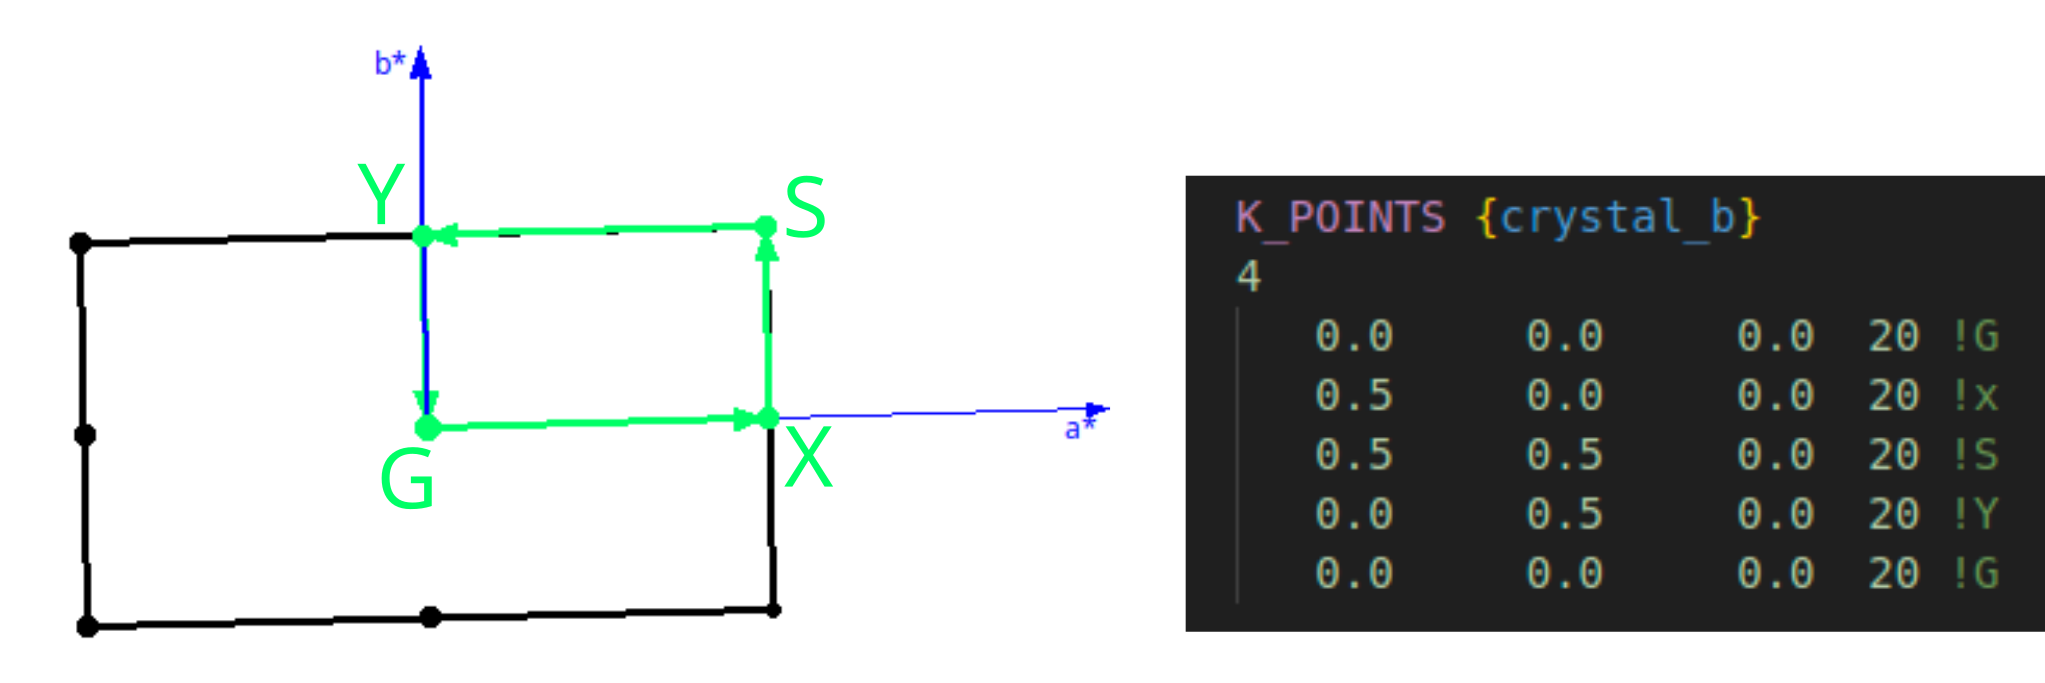
\includegraphics[width = 0.7\textwidth]{figs/ass1_WTe2_kpoints.png}
    \caption{The path along the high-symmetry points (left) and their coordinates with respect to the vectors of the Brillouin zone (right) used to calculate the electronic structure of a monolayer of WTe2. }
    \label{fig:ass1_kpoints}
  \end{figure}

Figure \ref{fig:ass1_bands}(a) shows the calculated band structure of the monolayer of WTe2. There is a significant difference between the two band diagrams which is likely due to different paths within the Brillouin zone, or a miscalculation of the Fermi energy. 
\begin{figure}[h]
    \centering 
    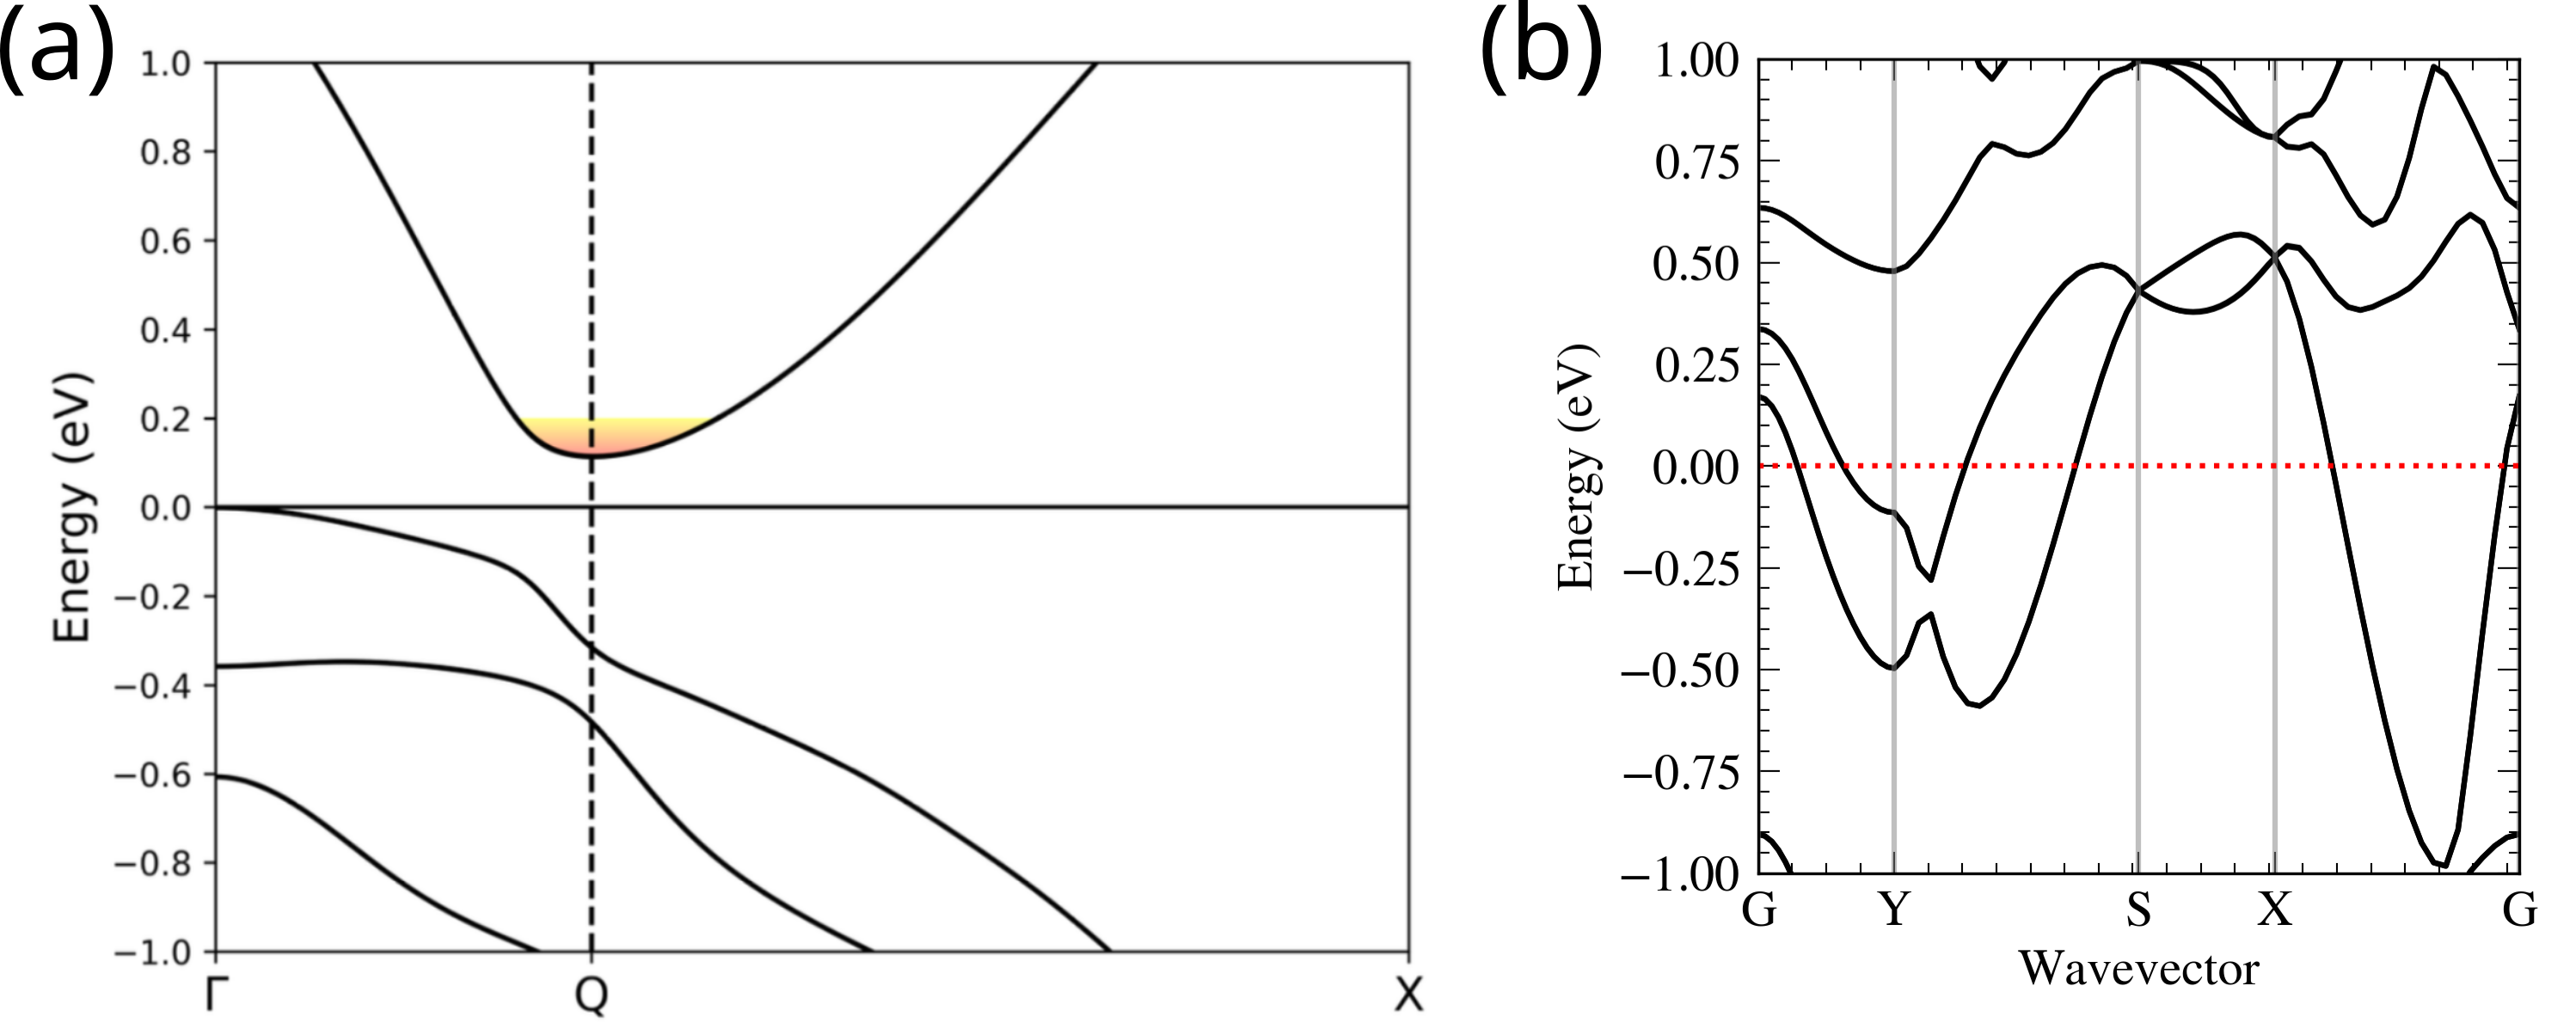
\includegraphics[width = 0.7\textwidth]{figs/ass1_bands_both.png}
    \caption{The band structure of a monolayer of WTe2 (a) given in the lecture slides and (b) calculated (right). The significant difference is likely due to a different symmetry path taken within the Brillouin zone.}
    \label{fig:ass1_bands}
  \end{figure}


\newpage
\section{Assignment 2: Graphene}
\subsection{Structure Construction}
The graphene monolayer was constructed in a similar fashion as the WTe2 monolayer.


Mainly, a hexagonal supercell was with lattice parameters $a=4.641$ Bohr and $c/a=4$. The parameter $a$ was chosen to match the optimized parameter found in week 2, while $c/a$ was chosen such that the distance between two monolayers is approximately 30 \AA.   
\begin{lstlisting}[ 
    caption={The \texttt{system} and \texttt{electrons} namespaces for the graphene monolayer.},
    label=lst:ass2_grapheneSyst,
    ]
&system    
  ibrav= 4,
  celldm(1)= 4.641, 
  celldm(3)= 13.0,   ! Approximately 30 angstrom between monolayers
  nat=  2, ntyp= 1, 
  ! Following copies what was done for  WTe2 file
  occupations = 'smearing', smearing = 'gaussian', degauss = 0.01,
  ecutwfc = 60.0,
  ecutrho = 600.0,
/
&electrons ! Same as week1 graphite
  mixing_mode = 'plain'
  mixing_beta = 0.7 
  conv_thr =  1.0d-8
/
\end{lstlisting}

To have a monolayer, only two carbon atoms were used and placed using the code in listing \ref{lst:ass2_grapheneAtoms}. The final graphene supercell is shown in Figure \ref{fig:ass2_graphene_cryst}
\begin{lstlisting}[ 
    caption={The \texttt{system} and \texttt{electrons} namespaces for the graphene monolayer.},
    label=lst:ass2_grapheneAtoms,
    ]
ATOMIC_SPECIES
  C  12.011  C.pbe-n-kjpaw_psl.1.0.0.UPF
ATOMIC_POSITIONS (alat)
  C      0.000 0.000 0.5
  C      0.000 0.577 0.5
\end{lstlisting}

\begin{figure}[h]
    \centering 
    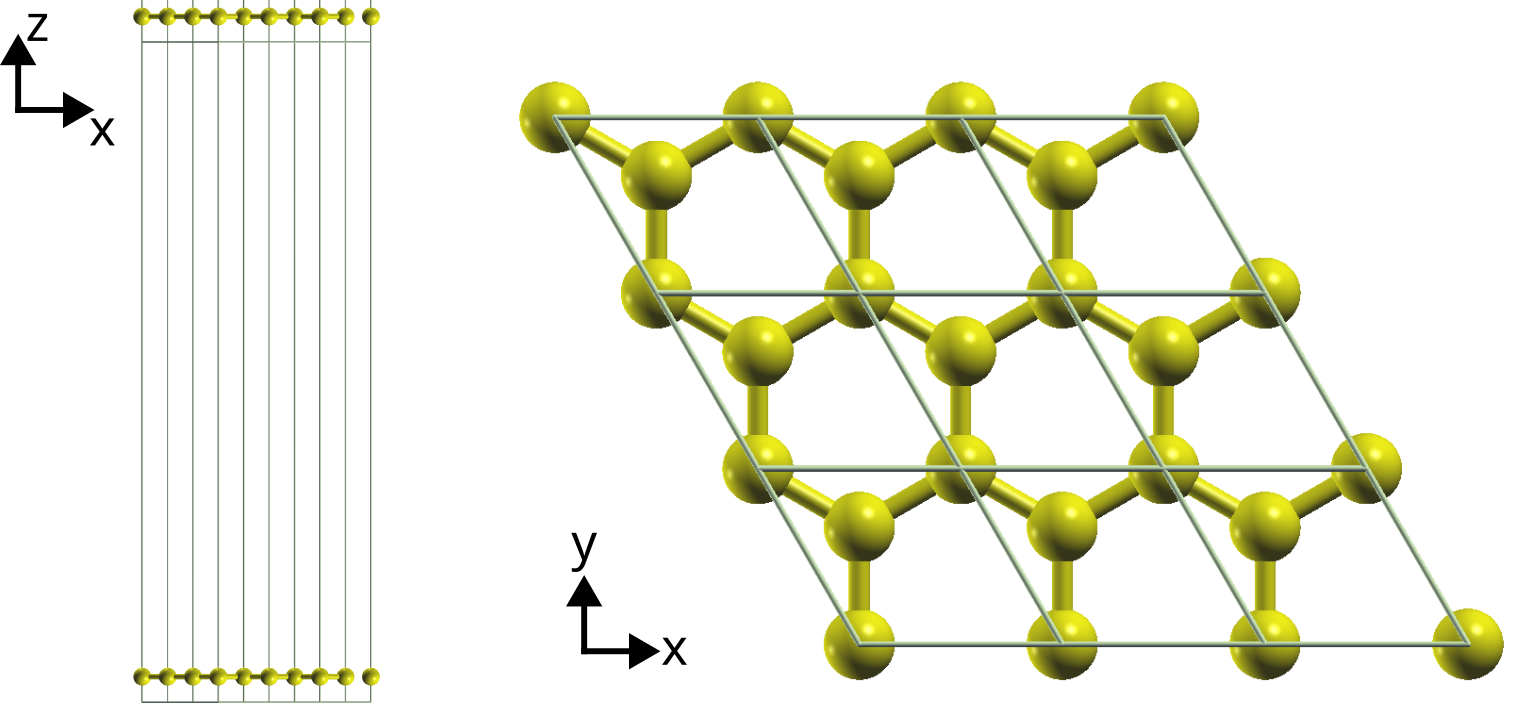
\includegraphics[width = 0.7\textwidth]{figs/ass2_graphene_struct.png}
    \caption{The \texttt{xcrysden} visualization of the graphene monolayer. The distance between two monolayers is approximately 30 \AA. as provided in the input file. }
    \label{fig:ass2_graphene_cryst}
  \end{figure}

\newpage
\subsection{Band Structure}
The high-symmetry point path chosen to outline the electronic structure of graphene is shown in Figure \ref{fig:ass2_kpoints}
\begin{figure}[h]
    \centering 
    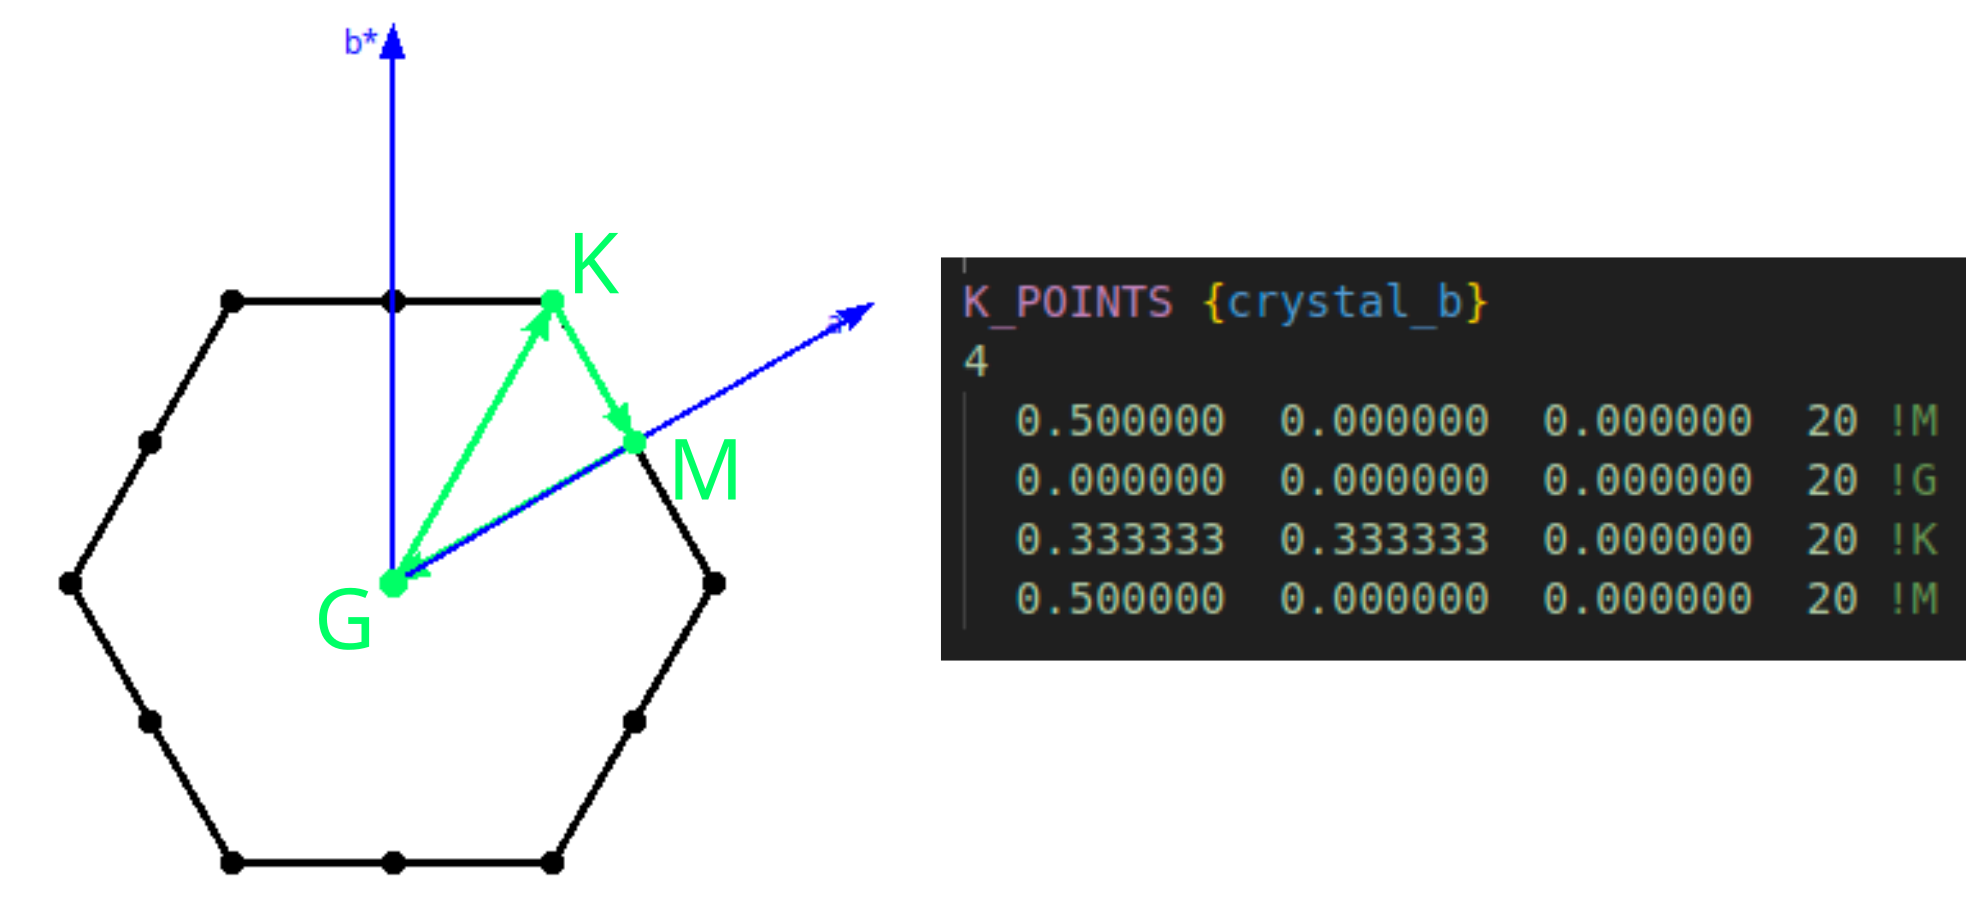
\includegraphics[width = 0.7\textwidth]{figs/ass2_graphene_kpoints.png}
    \caption{The path along the high-symmetry points (left) and their coordinates with respect to the vectors of the Brillouin zone (right) used to calculate the electronic structure of a monolayer of graphene. }
    \label{fig:ass2_kpoints}
  \end{figure}

Figure \ref{fig:ass2_bands}(a) shows the calculated band structures of graphite and graphene while Figure \ref{fig:ass2_bands}(b) shows band structures from literature \cite{newsonDynamicsCarriersPhotoinjected2010a}. In graphene, the certain bands in the M-G-K path combine to increase the degeneracy of the system. Furthermore, the formation of Dirac cones at point K is observed in the calculated band structure. However, the Fermi energy seems to be over-estimated.   
\begin{figure}[h!]
  \centering 
  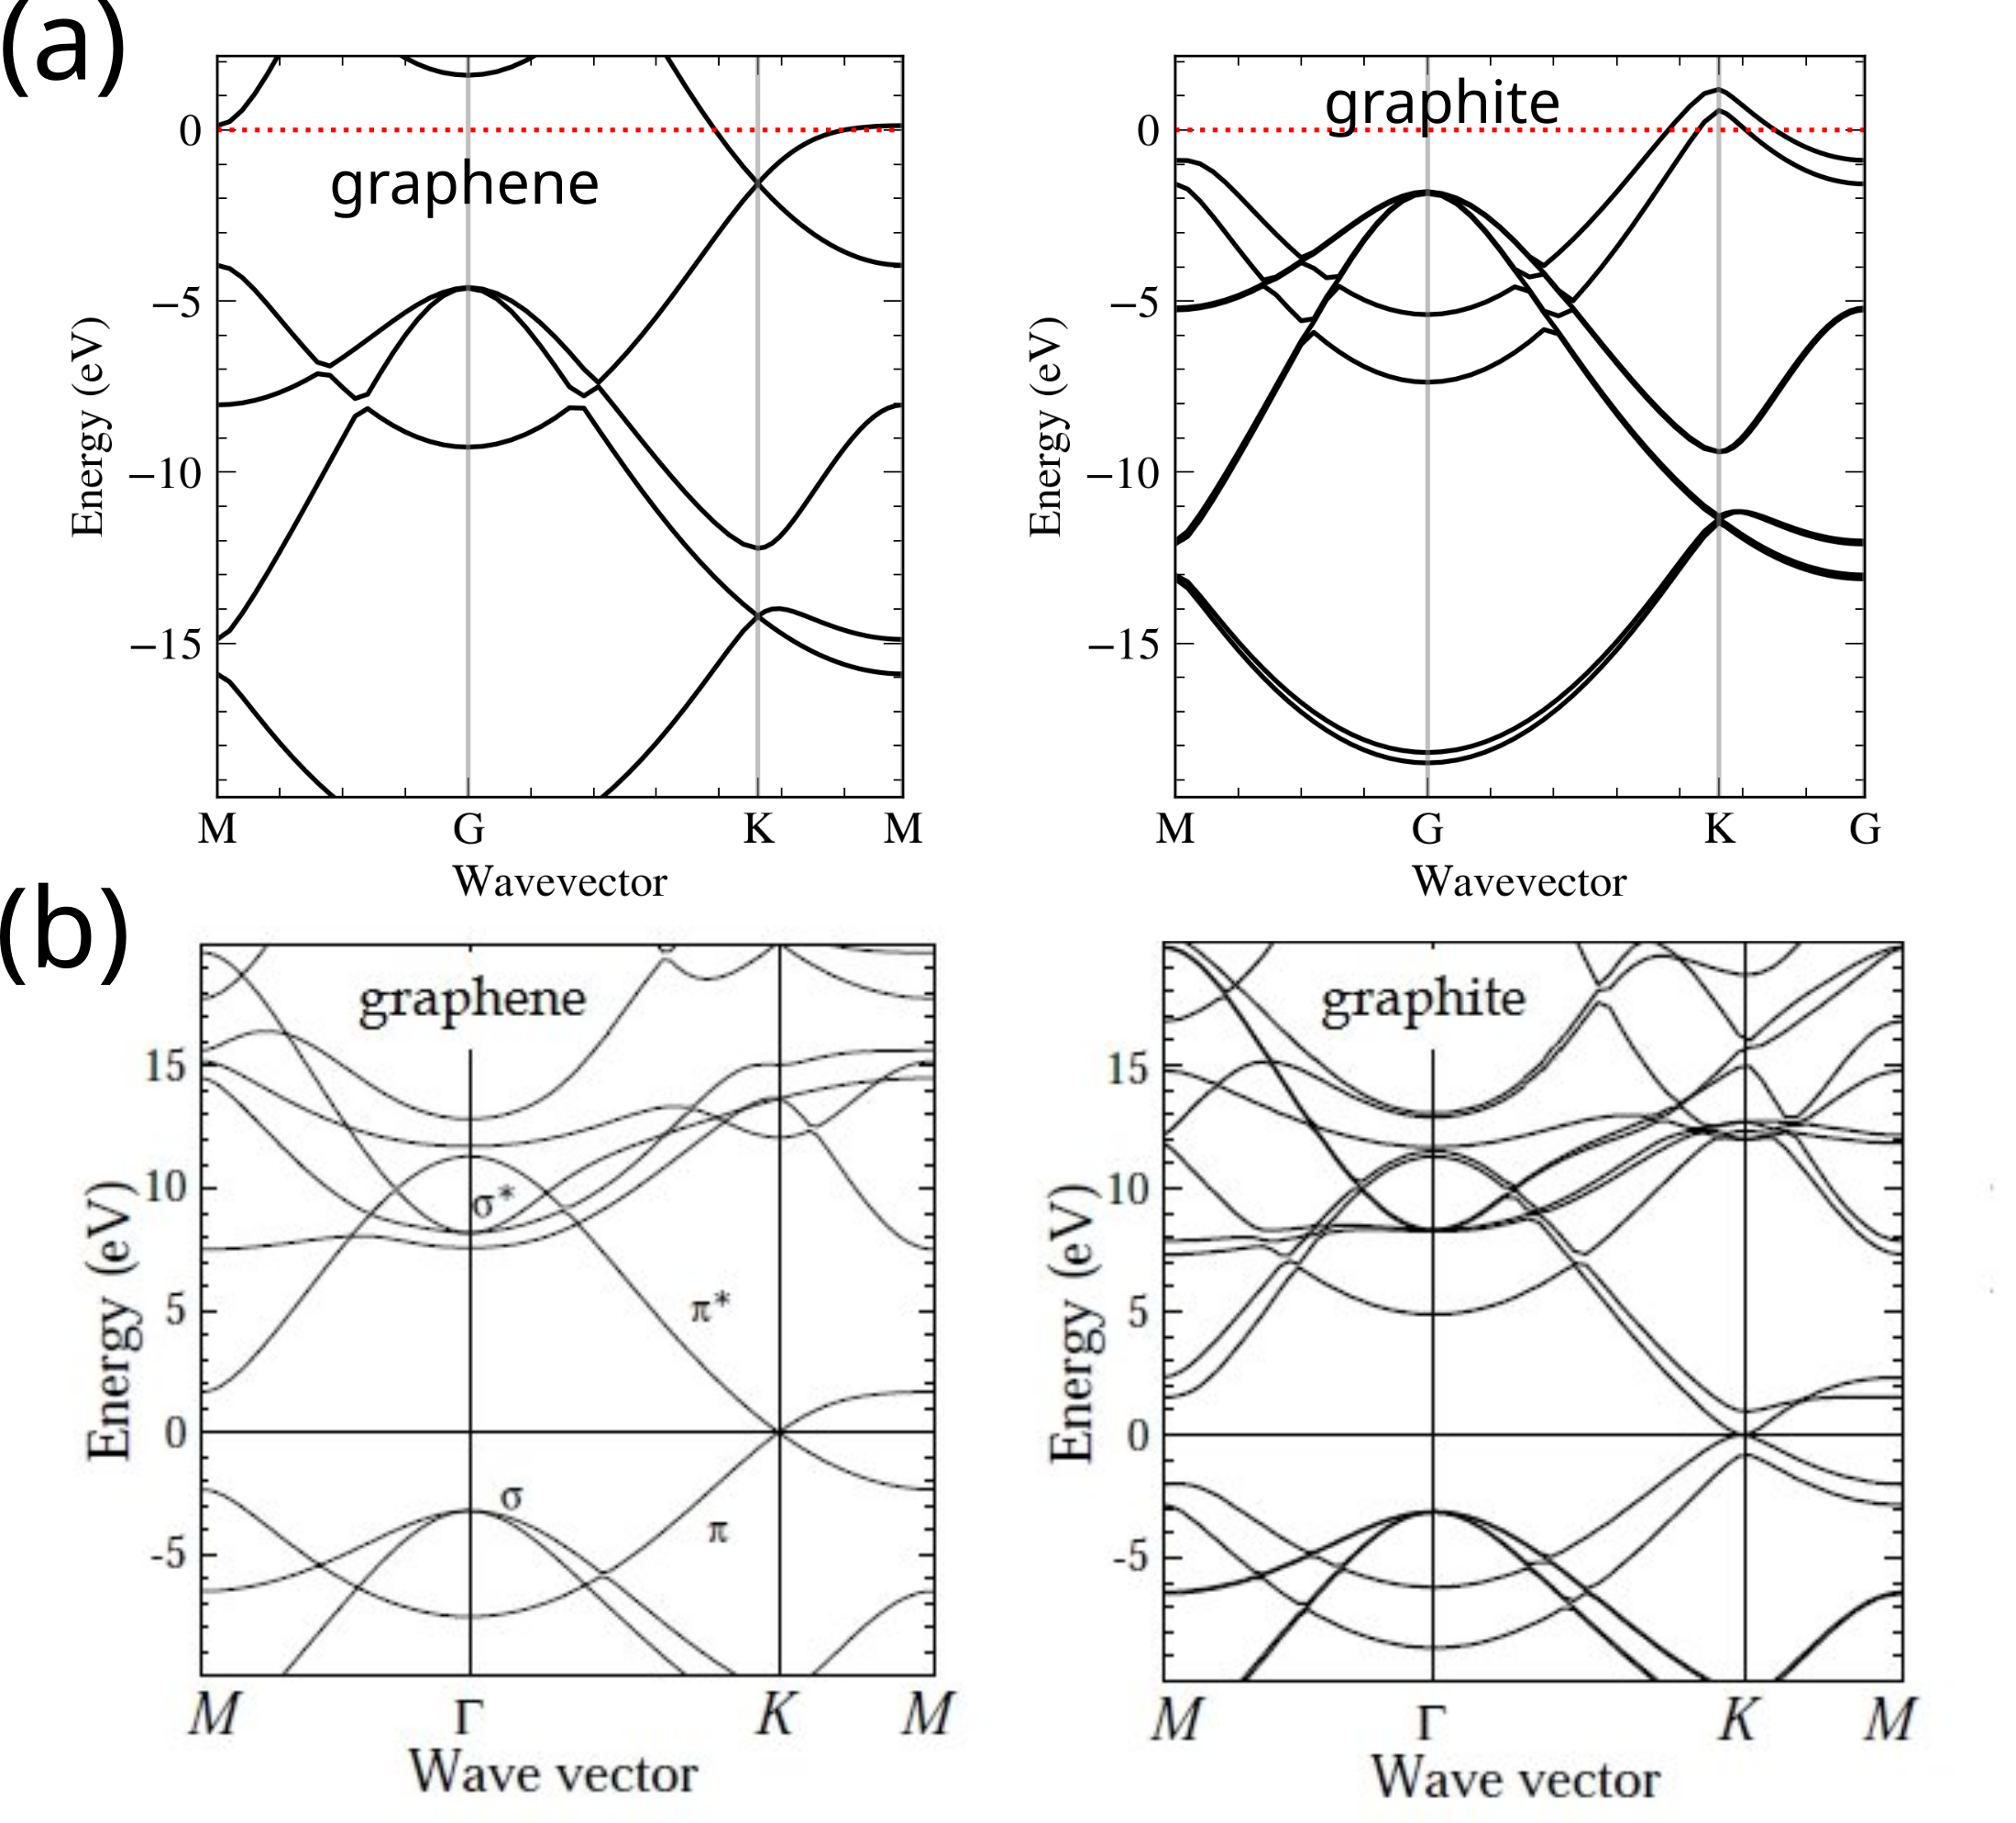
\includegraphics[width = 0.8\textwidth]{figs/ass2_graphene_bands.png}
  \caption{The band structure of graphene (left) and graphite (right) along the M-G-K-M path for (a) our calculations and (b) for literature \cite{newsonDynamicsCarriersPhotoinjected2010a}. The calculated band structures of both graphene and graphite are in relative agreement with the literature value, however the Fermi energy (red) is off in both calculations. }
  \label{fig:ass2_bands}
\end{figure}


\newpage 
\section{Assignment 3: Gr/WTe2 Heterostructure}
\subsection{Analysis of Given File}
The \texttt{xcrysden} visualization of the \texttt{wte2-gr.relax.in} is shown in Figure \ref{fig:ass3_struct1}. This visualization makes it clear that the supercell is rectangular and that there is a twisting angle of 90$^\circ$ between the two structures. Further consideration reveals that the supercell contains 40 graphene unit cells. The distance between the two monolayers is approximately 6.0 \AA, as determined from the graphene layer to the tungsten atoms.   

\begin{figure}[h!]
  \centering 
  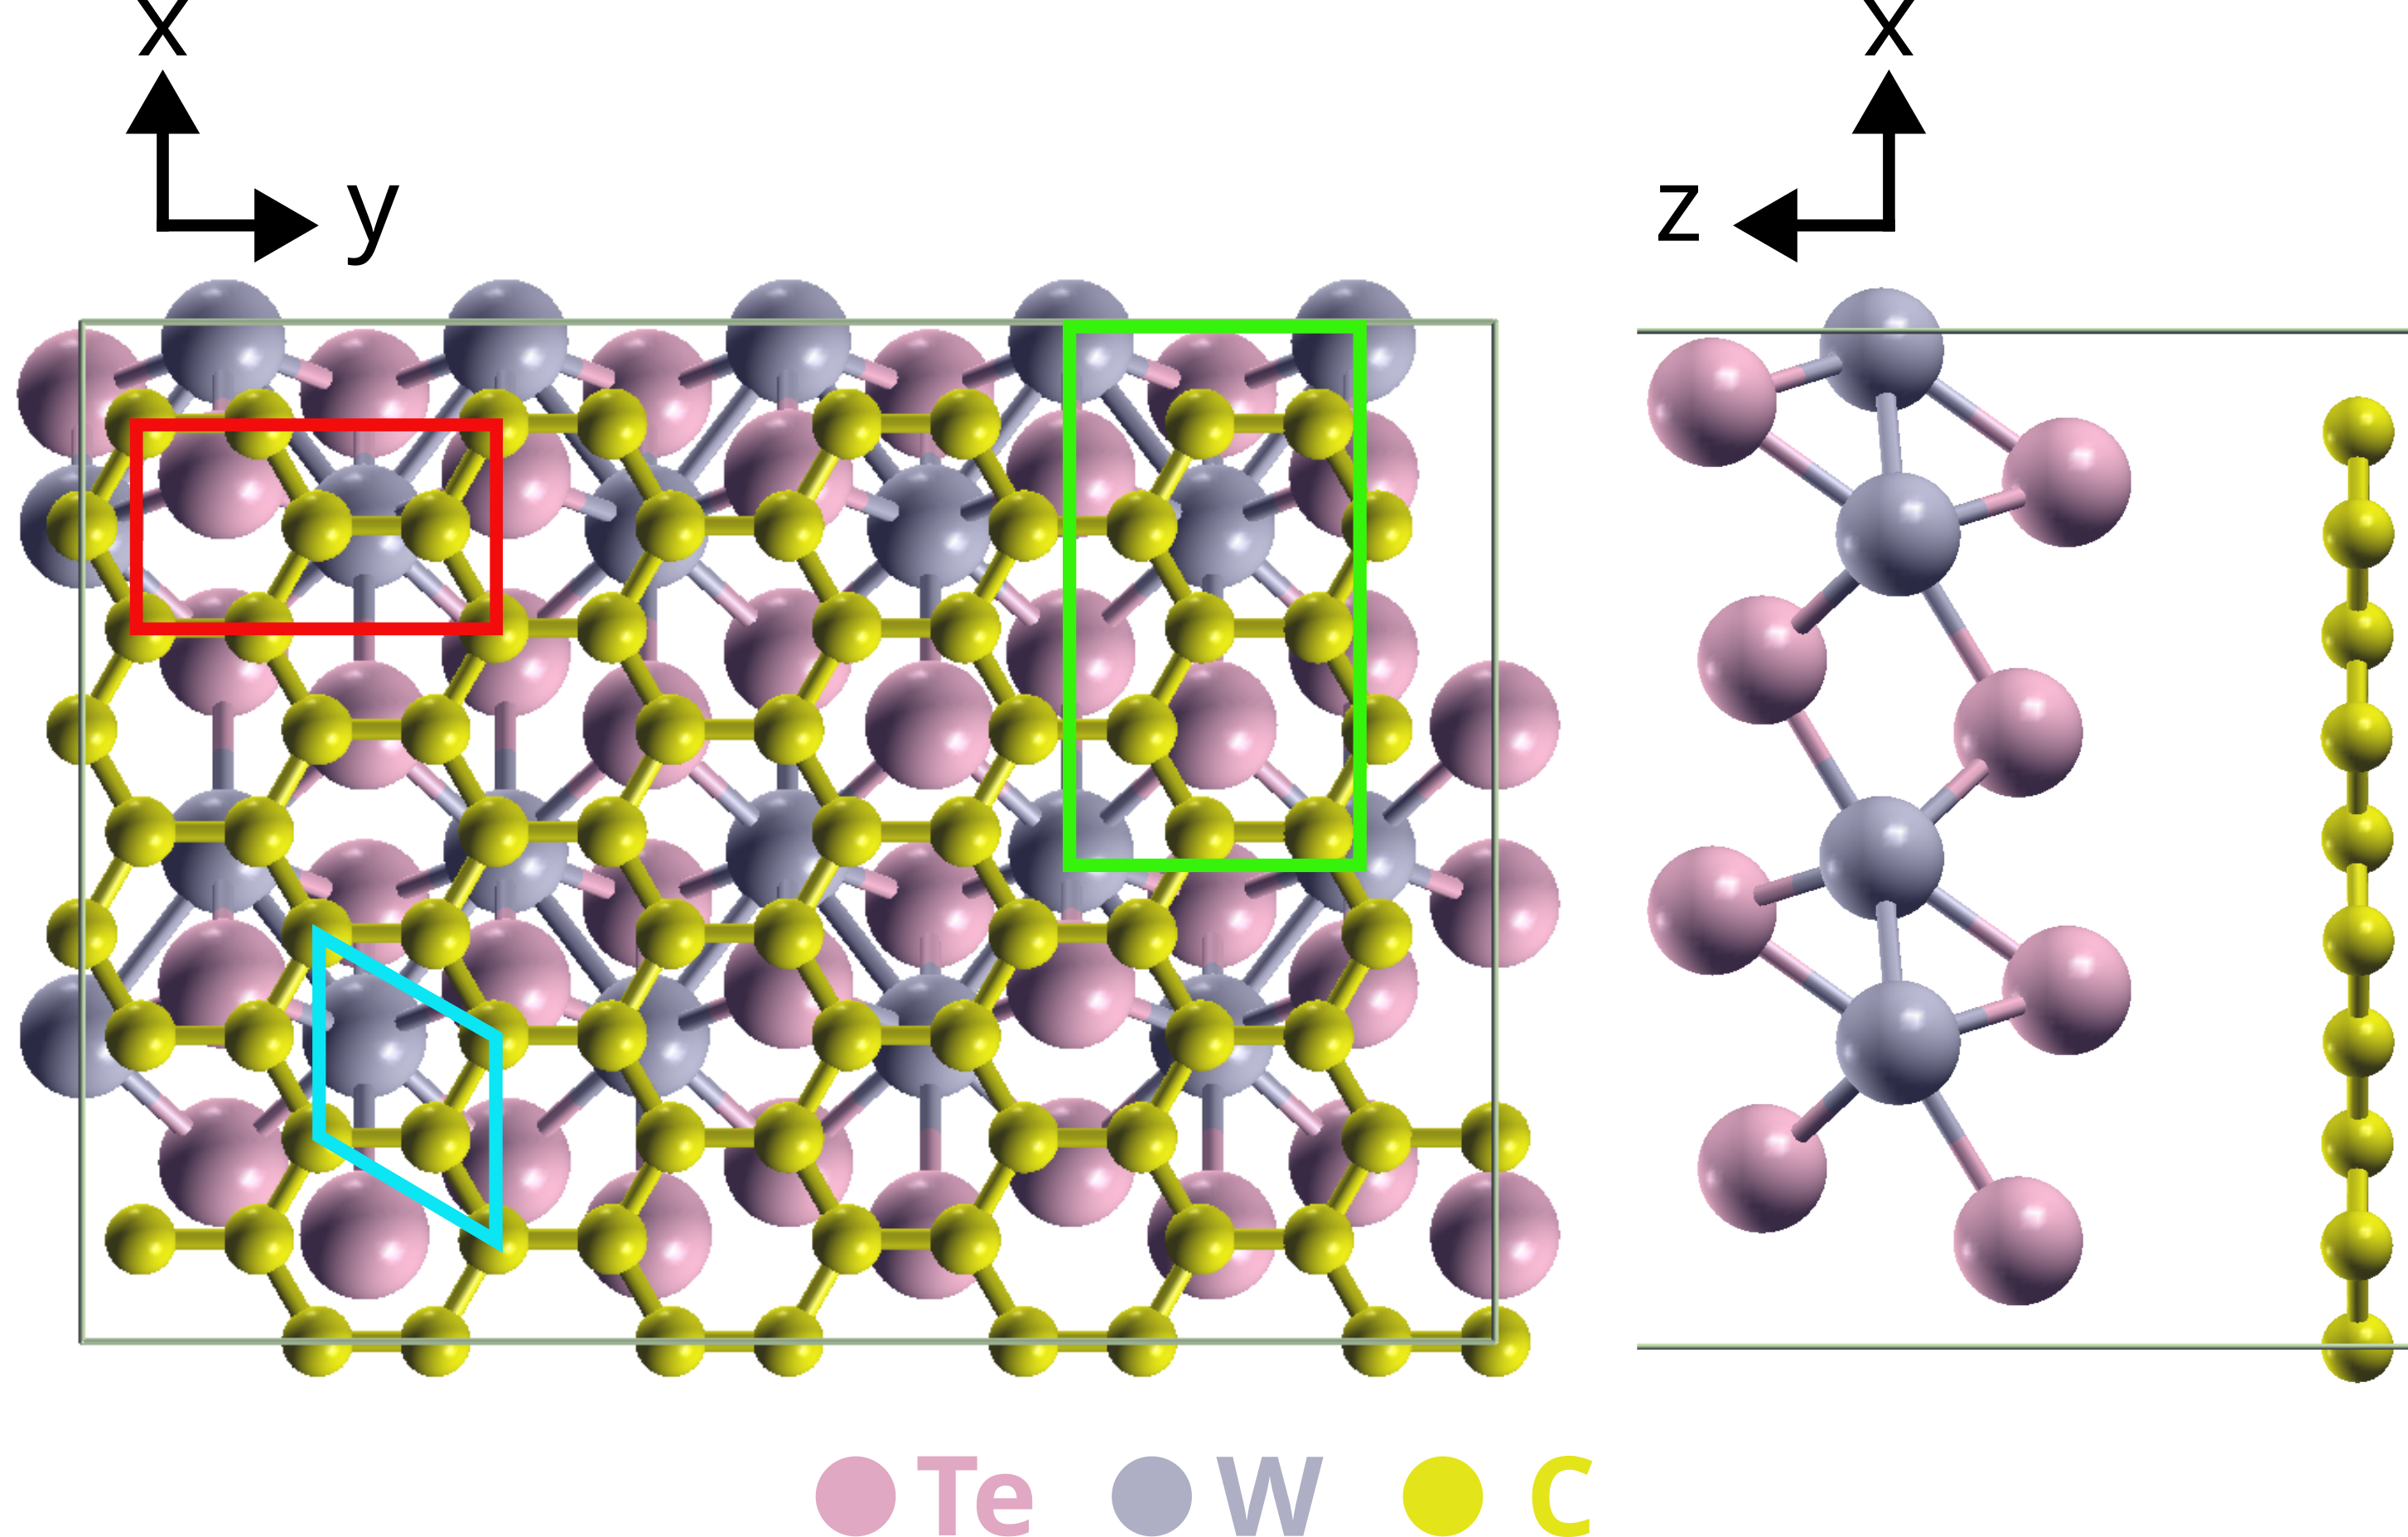
\includegraphics[width = 0.8\textwidth]{figs/gr-wte2_struct.png}
  \caption{The \texttt{xcrysden} visualization of the provided Gr-WTe2 supercell. The red rectangle shows a rectangular cell of graphene containing four carbon (yellow) atoms, while the blue rhombus represents a unit cell of graphene containing two atoms. The green rectangle shows the rectangular unit cell of WTe2. Comparison between the two unit cells shows that there is an angle of 90$^\circ$ between the two monolayers. The supercell contains 40 unit cells of graphene, but six unit cells of WTe2. }
  \label{fig:ass3_struct1}
\end{figure}



\subsection{Preparation of Heterostructure}
The preparation of the Gr/WTe2 heterostructure was completed by following the steps outlined by the video \url{https://youtu.be/vAc_vlSfQT0?si=nRrbpZ4OUzeHucB6}, and using the graphene and WTe2 supercells from the previous steps. This method is advantageous as it distributes the lattice mismatch throughout the entire crystal structure by saving the atom coordinates with fractional coordinates to \texttt{.vasp} file using \texttt{vesta}. 

The Main steps are outlined below, with the final structures shown in Figures \ref{fig:ass3_notwist_struct} and \ref{fig:ass3_twist_struct}.
\begin{enumerate}
  \item The first step was to transform the unit cell of graphene in to a rectangular unit cell, which was achieved using basic geometry and can be seen in Figure \ref{fig:ass3_grapheneRect}
  \begin{figure}[h!]
  \centering 
  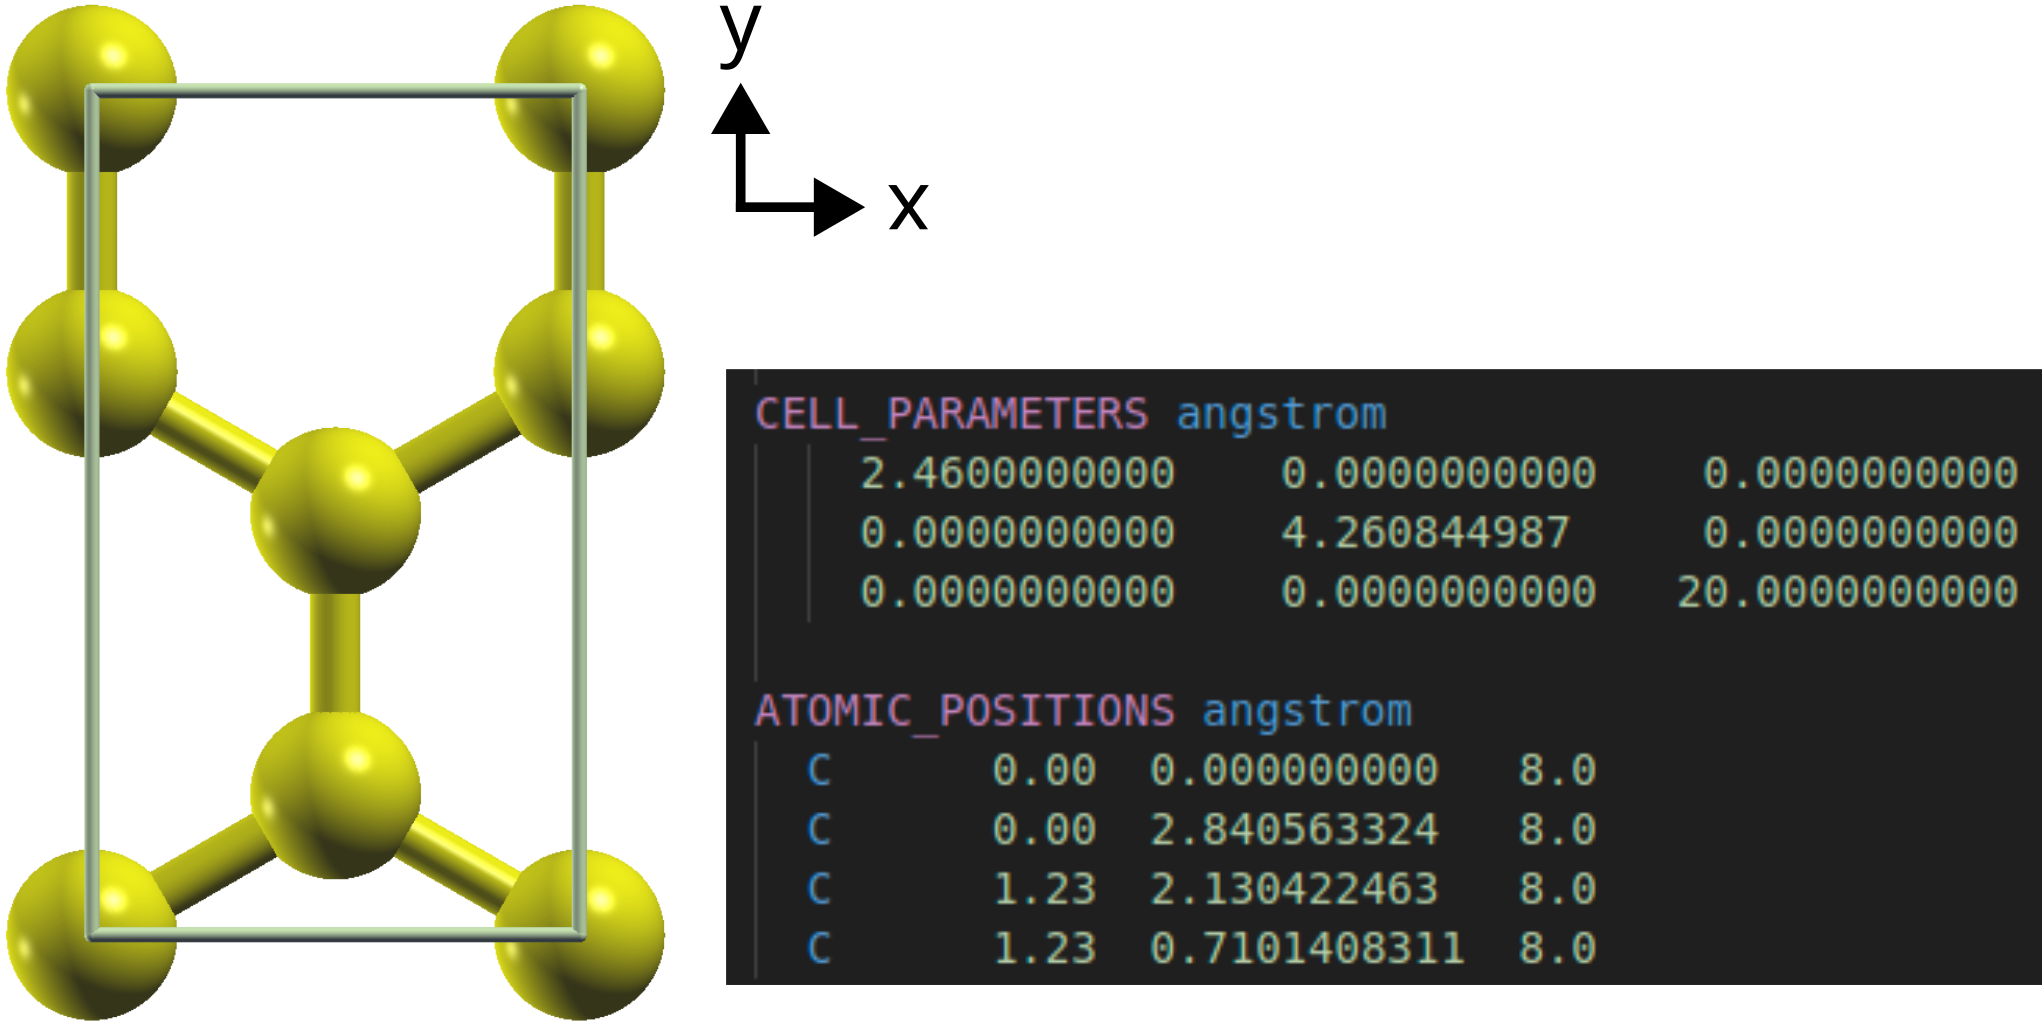
\includegraphics[width = 0.56\textwidth]{figs/ass3_grapheneRect.png}
  \caption{The \texttt{xcrysden} visualization (left) of a rectangular unit cell of graphene with the lattice parameters and atom coordinates (right).}
  \label{fig:ass3_grapheneRect}
\end{figure}

  \item The input files of each monolayer supercell were saved as \texttt{.xsf} files using \texttt{xcrysden} to allow the use of \texttt{vesta} to manipulate the crystal structures. 

  \item The supercells were then expanded using \texttt{vesta} to the least common multiple of both lattice sides. In the case of a twisting angle of 90$^\circ$, this corresponds to \texttt{graphene\_5x4x1} and \texttt{wte2\_90\_2x5x1} with the naming convention $a_x\times a_y \times a_z$. For no twisting angle, the expansions are {graphene\_3x6x1} and \texttt{wte2\_2x4x1}. See Figure \ref{fig:ass3_notwist_struct} and Figure \ref{fig:ass3_twist_struct} for clarification.  
  
  \item  The coordinates of each supercell were saved as a \texttt{.vasp} file with fractional coordinates. 
  
  \item The supercell parameters  of each supercell were set as the average between the expanded graphene and WTe2 supercells by editing the \texttt{.vasp} files, except for the z-coordinate. 
  This ensures that the supercells have the same lattice parameters. 
 
  \item A copy of one the supercells (I used WeT2) is then saved as the heterostructure \texttt{.vasp} file using \textbf{Cartesian coordinates}. The z-coordinate for this supercell was then set at 30 \AA. See listings \ref{lst:ass3_heterocell_notwist} and \ref{lst:ass3_heterocell_twist} for the final cell parameters for no twisting angle and with a $90^\circ$ twisting angle, respectively.
\begin{lstlisting}[ 
    caption={The cell parameters for the gr-wte2 supercell with no twisting angle. This was determined from the \texttt{graphene\_3x6x1} and \texttt{wte2\_2x4x1} expanded unit cells.},
    label=lst:ass3_heterocell_notwist,
    ]
CELL_PARAMETERS angstrom
    7.1900000570         0.0000000000         0.0000000000
    0.0000000000        25.3425359730         0.0000000000
    0.0000000000         0.0000000000        30.0000000000
\end{lstlisting}

\begin{lstlisting}[ 
    caption={The cell parameters for the gr-wte2 supercell with a twisting angle of 90$^\circ$. This was determined from the \texttt{graphene\_5x4x1} and \texttt{wte2\_90\_2x5x1} expanded unit cells.},
    label=lst:ass3_heterocell_twist,
    ]
CELL_PARAMETERS angstrom
    12.430000305         0.0000000000         0.0000000000
    0.0000000000        17.271689415         0.0000000000
    0.0000000000         0.0000000000        30.0000000000
\end{lstlisting} 
  \item  The graphene monolayer was imported to the WeT2 \texttt{.vasp} file and then moved in the z-direction such that there was no overlap between the two monolayers, determined form the filled-space visualization. 
  \item The atom coordinates were then saved as a \texttt{.xyz} file, which is then copied to the \texttt{ATOM\_COORDINATES} namespace in the input file. These coordinates were also copied into the heterostructure \texttt{.vasp} file prepared in step 6. 
  \item The \texttt{\&system} namespace was then adjusted to have the correct number of atoms.
\end{enumerate}

The final constructed heterostructures for no twisting angle and a twisting angle of 90$^\circ$ are shown in Figures \ref{fig:ass3_notwist_struct} and \ref{fig:ass3_twist_struct}, respectively. 

\begin{figure}[h!]
  \centering 
  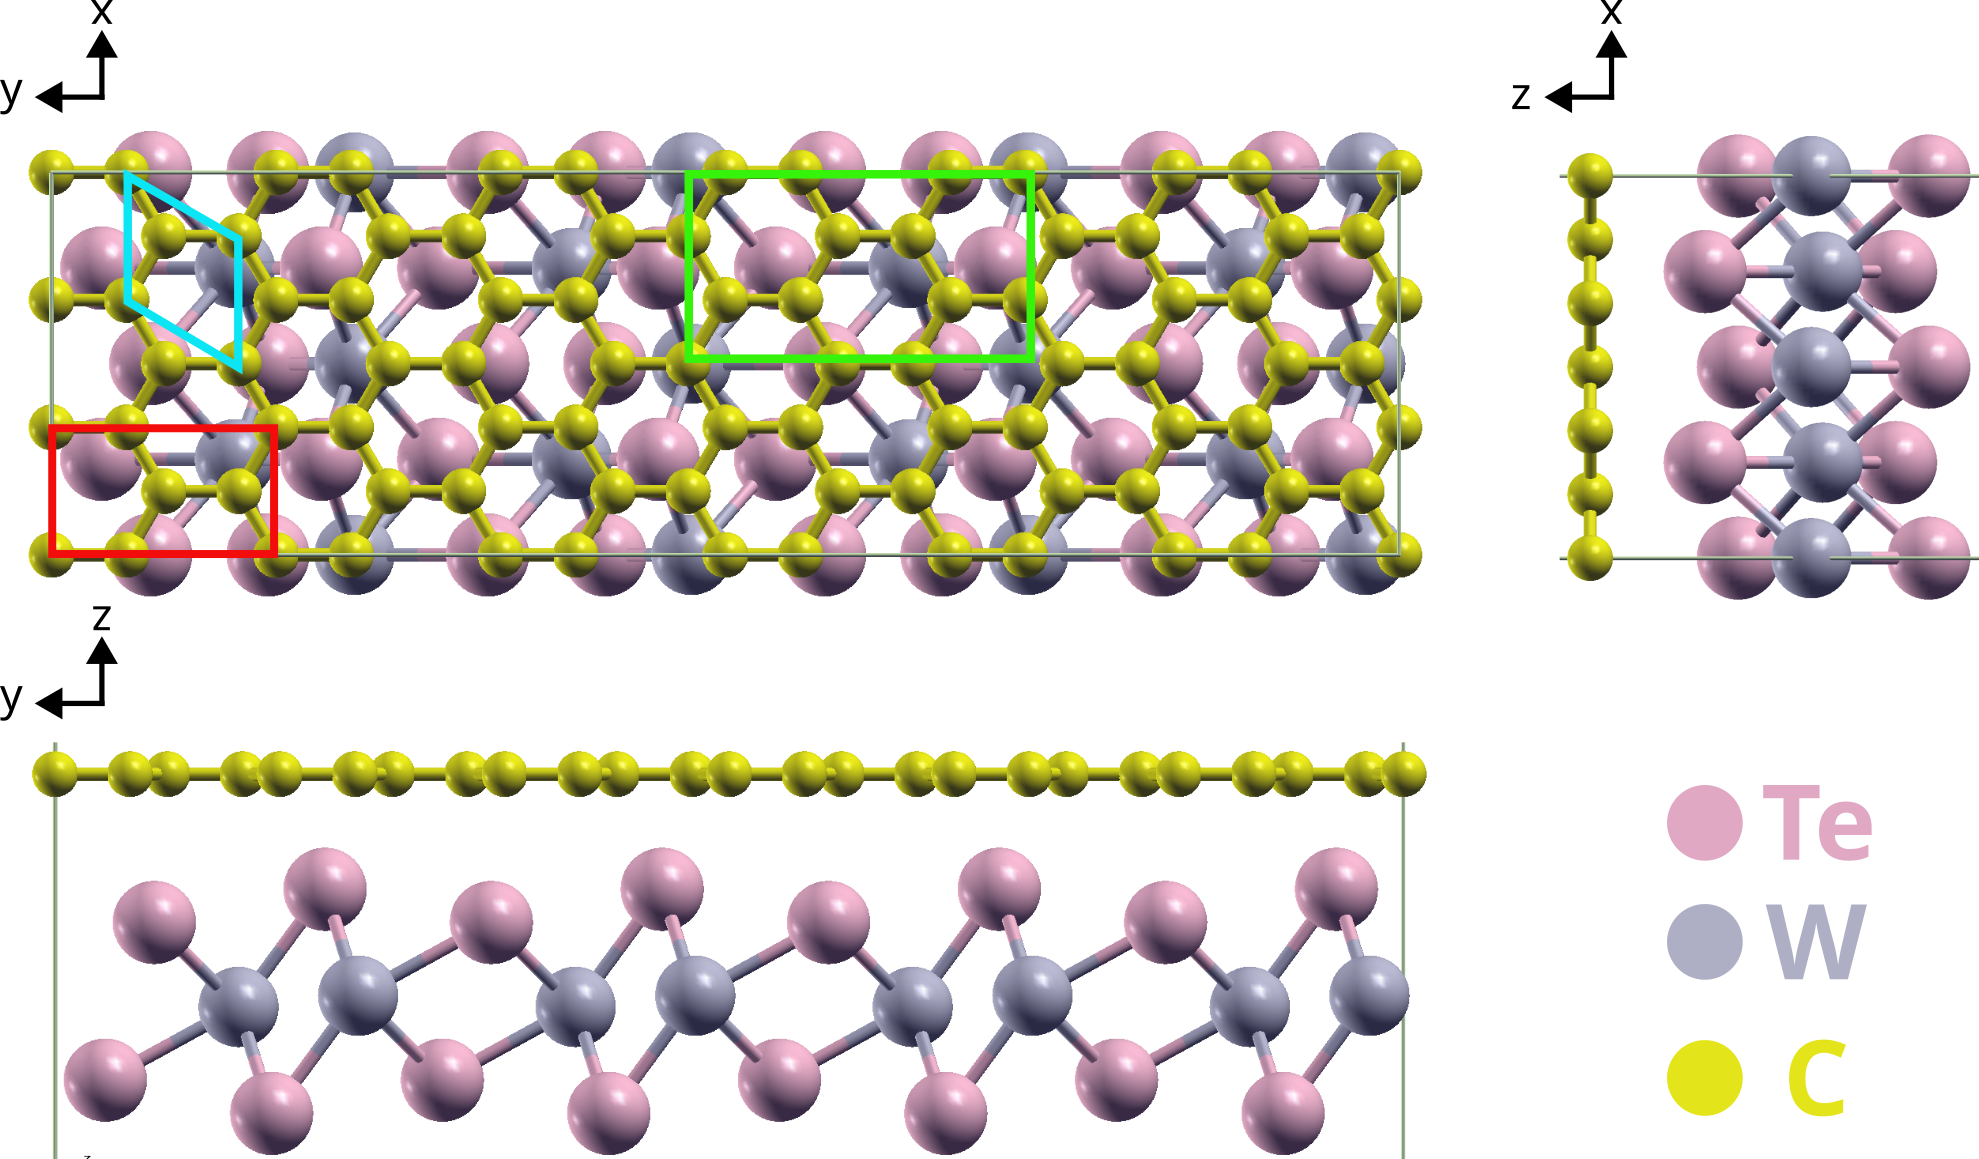
\includegraphics[width = 0.8\textwidth]{figs/ass3_notwist_struct.png}
  \caption{The \texttt{xcrysden} visualization of the constructed Gr-WTe2 supercell with no twisting angle. The red rectangle shows a rectangular cell of graphene containing four carbon (yellow) atoms, while the blue rhombus represents a unit cell of graphene containing two atoms. The green rectangle shows the rectangular unit cell of WTe2. The supercell contains 18 carbon rectangular cells and eight WTe2 unit cells. A total of 120 atoms are contained in this supercell. The distance between monolayers is determined to be about 4.2 \AA.}
  \label{fig:ass3_notwist_struct}
\end{figure}

\begin{figure}[h!]
  \centering 
  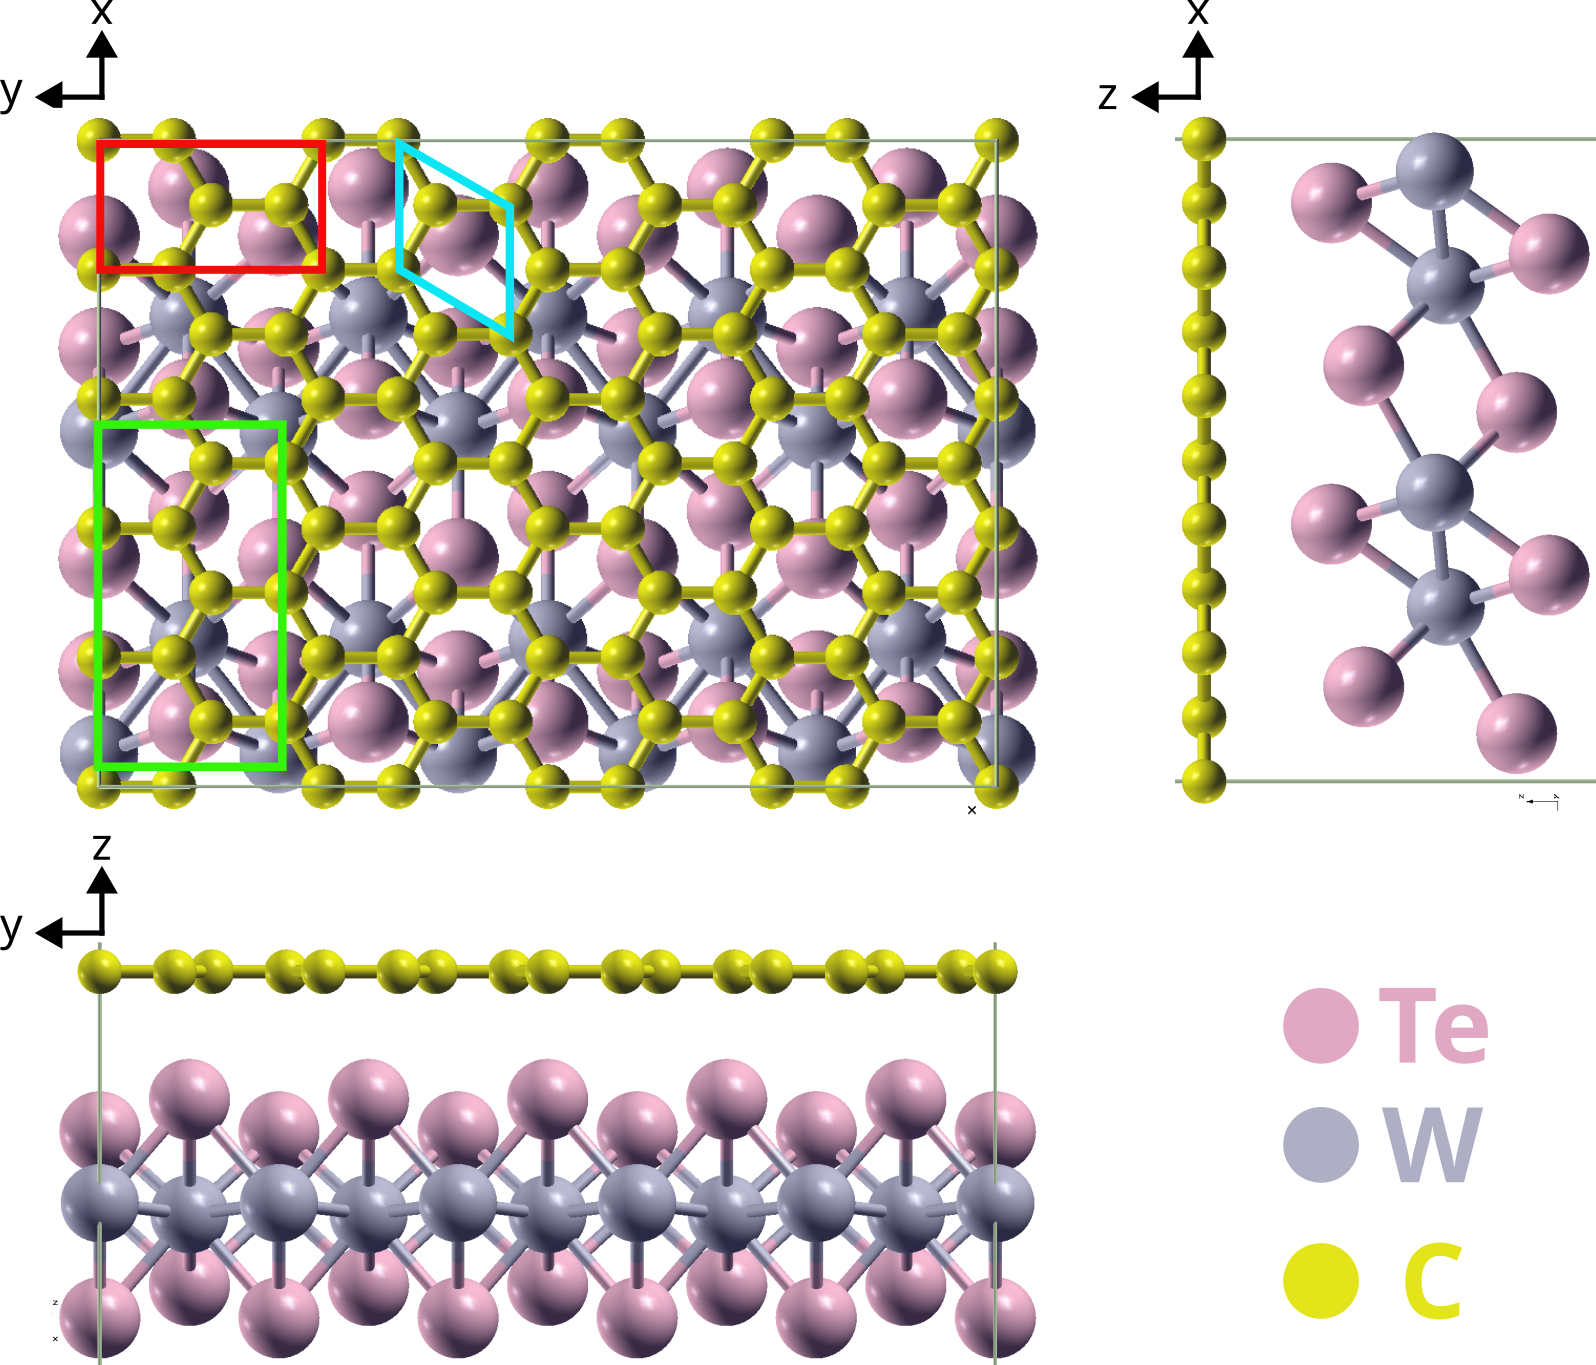
\includegraphics[width = 0.7\textwidth]{figs/ass3_twist_struct.png}
  \caption{The \texttt{xcrysden} visualization of the constructed Gr-WTe2 supercell with a twisting angle of 90$^\circ$. The red rectangle shows a rectangular cell of graphene containing four carbon (yellow) atoms, while the blue rhombus represents a unit cell of graphene containing two atoms. The green rectangle shows the rectangular unit cell of WTe2. The supercell contains 20 carbon rectangular cells and ten WTe2 unit cells. A total of 140 atoms are contained in this supercell. The distance between monolayers was determined to be about 4.7 \AA.}
  \label{fig:ass3_twist_struct}
\end{figure}

 \newpage
 \section{Assignment 4: Relaxing Heterostructure}
The Heterostructure with a twisting angle of 90$^\circ$ was chosen for the relaxation. 

In order for the relaxation to run, the \texttt{\&ions} namespace needed to be added to the input file provided on GitHub. The default values were used as shown in listing \ref{lst:ass4_ions}.  
\begin{lstlisting}[ 
    caption={The \texttt{ions} and namespace used for the Gr/WeT2 heterostructure relaxation.},
    label=lst:ass4_ions,
    ]
&ions
   ion_velocities = 'default',
   ion_dynamics = 'bfgs',
/
\end{lstlisting}
The \texttt{electrons} namespace used is shown in listing \ref{lst:ass4_electrons}. The relaxation was run on the parallel partition on a full node, but did not reach convergence after 80 electronic iterations. Nonetheless, the initial configuration and final configuration after 80 electronic iterations is shown in Figure \ref{fig:ass4_final_struct}
\begin{lstlisting}[ 
    caption={The \texttt{electrons} and namespace used for the Gr/WeT2 heterostructure relaxation.},
    label=lst:ass4_electrons,
    ]
&electrons
   mixing_beta = 0.9,
   mixing_mode = 'local-TF',
   conv_thr = 1.0d-9,
   electron_maxstep = 80,
/
\end{lstlisting} 
\begin{figure}[h!]
  \centering 
  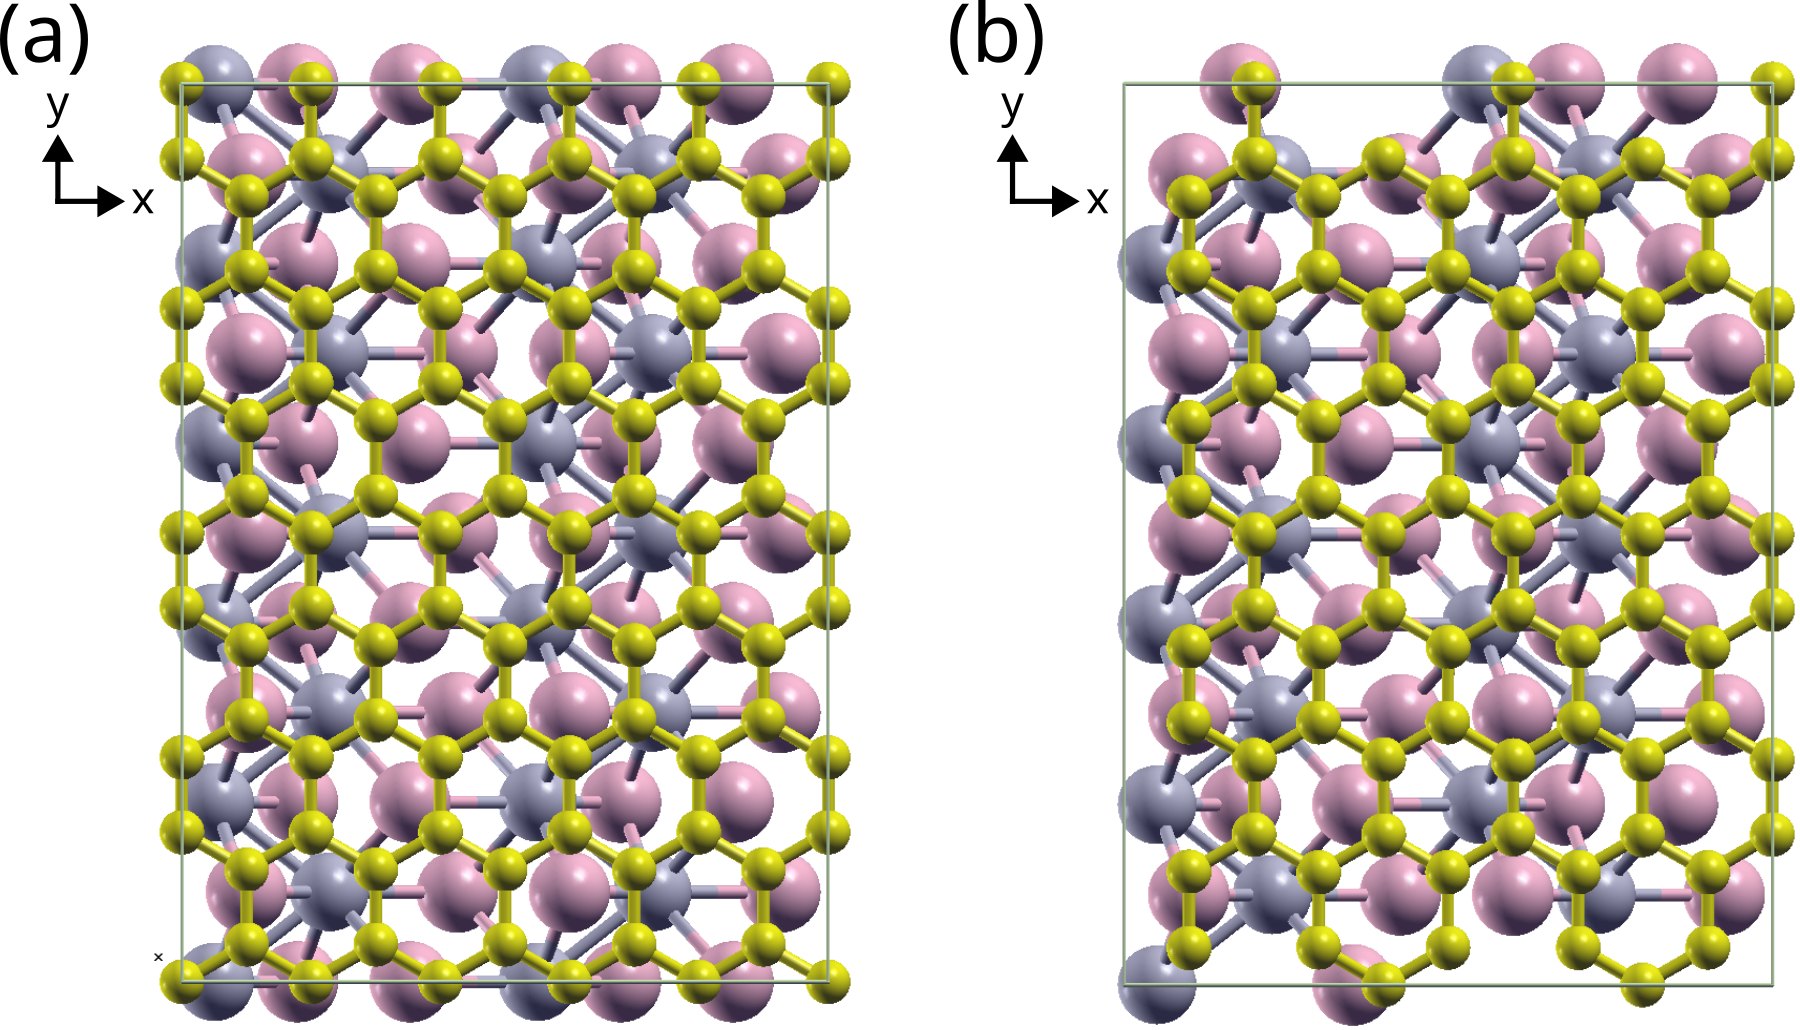
\includegraphics[width = 0.7\textwidth]{figs/ass4_final_struct.png}
  \caption{The \texttt{xcrysden} visualization of the constructed Gr-WTe2 supercell with a twisting angle of 90$^\circ$ (a) before relaxation (b) after 80 electronic iterations. The positions of the atoms have moved considerably.}
  \label{fig:ass4_final_struct}
\end{figure}





\printbibliography

% \begin{appendices}
%   \input{Appendix}
% \end{appendices}

\end{document}



